
\documentclass{beamer}

\usetheme{CambridgeUS}
%\usecolortheme{albatross}

\usepackage{graphicx} 
\usepackage{booktabs} 

\title[Week 1 Review]{EPSRC Vacation Scheme: Week 1 Review} 

\author{Matthew Knowles} 
\institute[UoY] 
{
Department of Mathematics \\
University of York \\ 
\medskip
\textit{mk1320@york.ac.uk} 
}
\date{$26^{th}$ July 2021} 

\begin{document}

\begin{frame}
\titlepage 
\end{frame}



\begin{frame}
\frametitle{Goals of last week}
\begin{enumerate}
	\item Implement 'by eye' algorithm for finding convex hull of piecewise linear functions.
	\pause
	\item Look around in literature to see what I could find.
\end{enumerate}
\end{frame}

\begin{frame}
\frametitle{Task 1 Progress}
\begin{itemize}
	\item Wrote this in roughly 60 lines of code
	\pause
	\item Tested on a few test datasets. Here are those results
	\pause
	\item You will notice that they are not perfect
\end{itemize}
\end{frame}

\begin{frame}
\frametitle{First test}
	\begin{figure}
		\center
		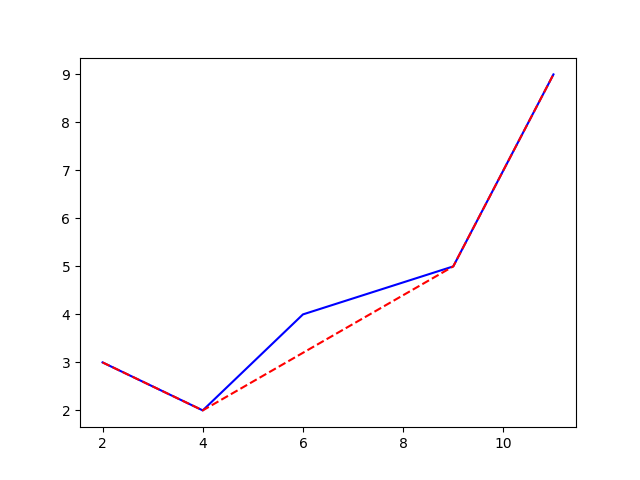
\includegraphics[scale=0.6]{../Figures/Figure_2.png}
	\end{figure}
\end{frame}

\begin{frame}
\frametitle{Slightly larger test}
	\begin{figure}
		\center
		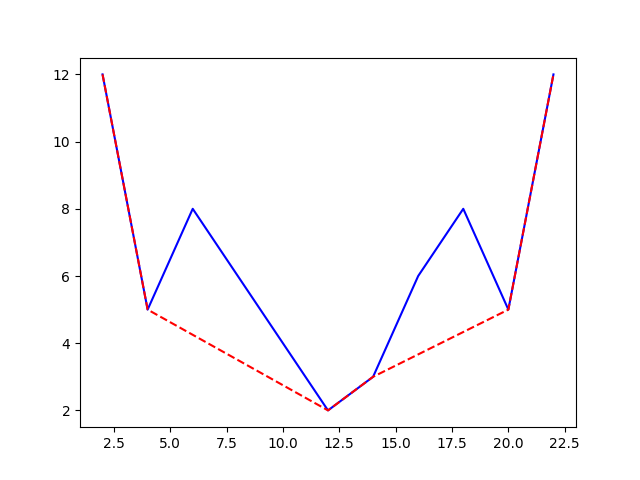
\includegraphics[scale=0.6]{../Figures/Figure_1.png}
	\end{figure}
\end{frame}

\begin{frame}
\frametitle{Test with 100 data points}
	\begin{figure}
		\center
		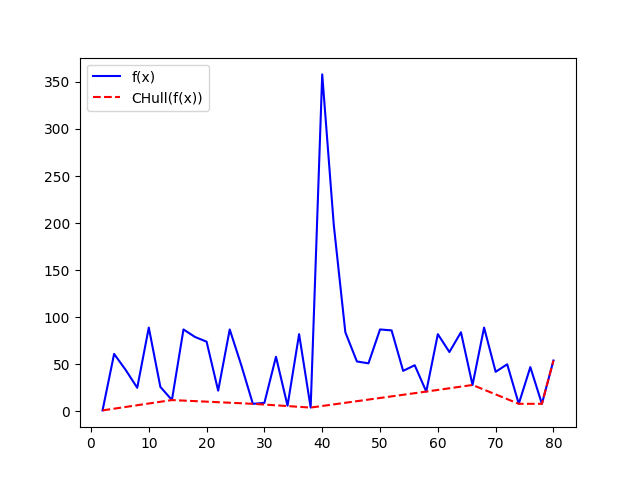
\includegraphics[scale=0.6]{../Figures/Figure_4.png}
	\end{figure}
\end{frame}

\begin{frame}
\frametitle{Test with 200 data points}
	\begin{figure}
		\center
		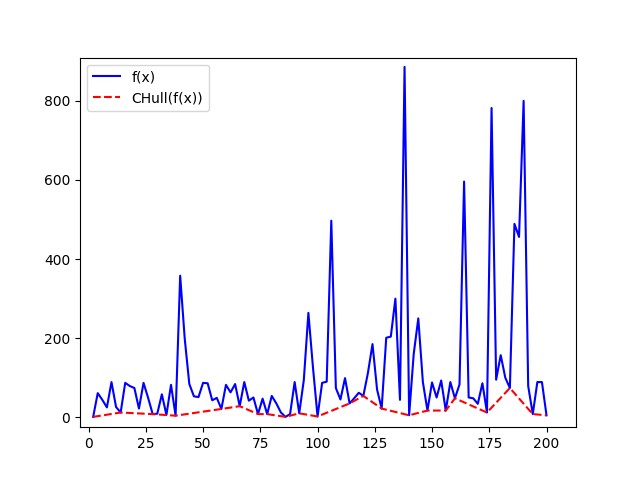
\includegraphics[scale=0.6]{../Figures/Figure_3.png}
	\end{figure}
\end{frame}

\begin{frame}
\frametitle{Problems}
\begin{itemize}
	\item Notice how the function it computes isn't entirely convex
	\pause
	\item Can remove this issue by recursively running through the hull
	\pause
	\item issue: this is going to get increasingly slower and slower
	\pause 
	\item Solution? Try another algo!
\end{itemize}
\end{frame}

\begin{frame}
\frametitle{Monotone Chain}
\begin{itemize}
	\item The Monotone Chain Algorithm runs in $\mathcal{O}(n \log n)$ time
	\pause 
	\item Usually runs a sub-routine on upper and lower part of the set, we are only interested in the lower part however
	\pause
	\item Only looking at one hull reduces to $\mathcal{O}(n)$ complexity
\end{itemize}
\end{frame}

\begin{frame}
	\begin{figure}
		\center
		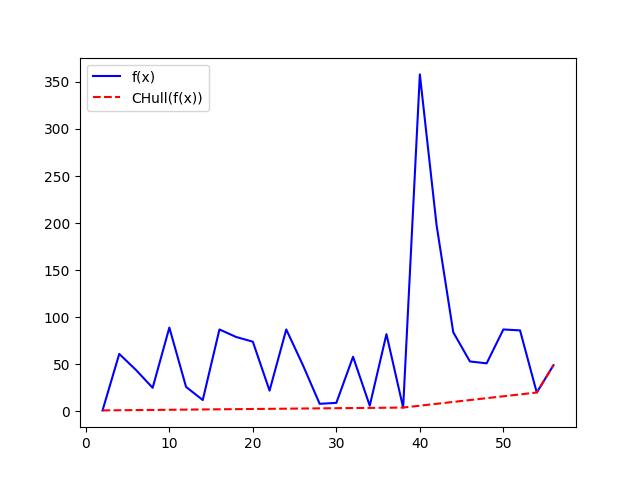
\includegraphics[scale=0.6]{../Figures/Figure_5.png}
	\end{figure}
\end{frame}

\begin{frame}
\Huge{\centerline{Any Questions?}}
\end{frame}


\end{document} 